\documentclass[12pt]{book}
\setlength{\headheight}{15pt}

\usepackage[margin=1in]{geometry}
\usepackage{color, colortbl}
\usepackage{fancyhdr}
\usepackage{amssymb}
\usepackage{amsmath}
\usepackage{lastpage}
\usepackage{karnaugh-map}
\usepackage{multicol}
\usepackage{graphicx}

\graphicspath{ {./graphics/} }

% begin custom header shit
\pagestyle{fancy}
\fancyhf{}
\lhead{COMP2650 Lecture 9 - Combinational Logic}
\rhead{Isaac Kilbourne (110043640)}
\rfoot{Page \thepage\ of \pageref{LastPage}}
% end custom header shit

\definecolor{LightRed}{rgb}{1, 0.6, 0.6}
\definecolor{LightGreen}{rgb}{0.6, 1, 0.6}
\newcolumntype{R}{>{\columncolor{LightRed}}c}
\newcolumntype{G}{>{\columncolor{LightGreen}}c}

\newenvironment{indented}[1] {
	\begin{list}{}{\setlength{\leftmargin}{#1}}
		\item[]
	}{\end{list}}
	
\raggedbottom 
\begin{document}
	\noindent
	2. Design an Excess3-to-Aiken decoder in the form of product of sums.
	\begin{indented}{5mm}
		$\begin{array}{c|c|c|c||c|c|c|c||c}
			A & B & C & D & F1 & F2 & F3 & F4 & \#\\
			\hline
		  % A   B   C   D   F1  F2  F3  F4  #
			0 & 0 & 0 & 0 & X & X & X & X & 0\\
			0 & 0 & 0 & 1 & X & X & X & X & 1\\
			0 & 0 & 1 & 0 & X & X & X & X & 2\\
			0 & 0 & 1 & 1 & 0 & 0 & 0 & 0 & 3\\
			0 & 1 & 0 & 0 & 0 & 0 & 0 & 1 & 4\\
			0 & 1 & 0 & 1 & 0 & 0 & 1 & 0 & 5\\
			0 & 1 & 1 & 0 & 0 & 0 & 1 & 1 & 6\\
			0 & 1 & 1 & 1 & 0 & 1 & 0 & 0 & 7\\
			1 & 0 & 0 & 0 & 1 & 0 & 1 & 1 & 8\\
			1 & 0 & 0 & 1 & 1 & 1 & 0 & 0 & 9\\
			1 & 0 & 1 & 0 & 1 & 1 & 0 & 0 & 10\\
			1 & 0 & 1 & 1 & 1 & 1 & 1 & 0 & 11\\
			1 & 1 & 0 & 0 & 1 & 1 & 1 & 1 & 12\\
			1 & 1 & 0 & 1 & X & X & X & X & 13\\
			1 & 1 & 1 & 0 & X & X & X & X & 14\\
			1 & 1 & 1 & 1 & X & X & X & X & 15\\
		\end{array}$

		\begin{multicols}{2}
			\begin{karnaugh-map}[4][4][1][(F1) \ CD][AB]
				\minterms{3, 4, 5, 6, 7}
				\maxterms{8, 9, 10, 11, 12}
				\terms{0, 1, 2, 13, 14, 15}{X}

				\implicant{0}{6}
			\end{karnaugh-map}\\
			\begin{karnaugh-map}[4][4][1][(F3) \ CD][AB]
				\minterms{3,7,9,10}
				\maxterms{4, 5, 6, 8, 11, 12}
				\terms{0, 1, 2, 13, 14, 15}{X}
	
				\implicant{3}{7}
				\implicant{13}{9}
				\implicant{14}{10}
			\end{karnaugh-map}\\
			\begin{karnaugh-map}[4][4][1][(F2) \ CD][AB]
				\minterms{3, 4, 5, 6, 8}
				\maxterms{7, 9, 10, 11, 12}
				\terms{0, 1, 2, 13, 14, 15}{X}

				\implicant{0}{2}
				\implicant{0}{5}
				\implicant{2}{6}
				\implicantedge{0}{0}{8}{8}
			\end{karnaugh-map}\\
			\begin{karnaugh-map}[4][4][1][(F4) \ CD][AB]
				\minterms{3,5,7,9,10,11}
				\maxterms{4, 6, 8, 12}
				\terms{0, 1, 2, 13, 14, 15}{X}

				\implicant{0}{2}
				\implicant{1}{11}
				\implicant{15}{10}
			\end{karnaugh-map}
		\end{multicols}
		
		$\begin{aligned}
			\therefore F1 &= (A')'\\ 
			&= A
		\end{aligned}$

		$\begin{aligned}
			\therefore F2 &= ((A'B') + (A'C')' + (A'CD')' + (B'C'D'))'\\
			&= (A+B)(A+C)(A+C'+D)(B+C+D)
		\end{aligned}$

		$\begin{aligned}
			\therefore F3 &= ((A'CD)+(AC'D)+(ACD'))'\\
			&= (A+C'+D)(A'+C+D')(A'+C'+D)
		\end{aligned}$

		$\begin{aligned}
			\therefore F4 &= ((A'B')+(D)+(AC))'\\
			&= (A+B)(D')(A'+C')
		\end{aligned}$

		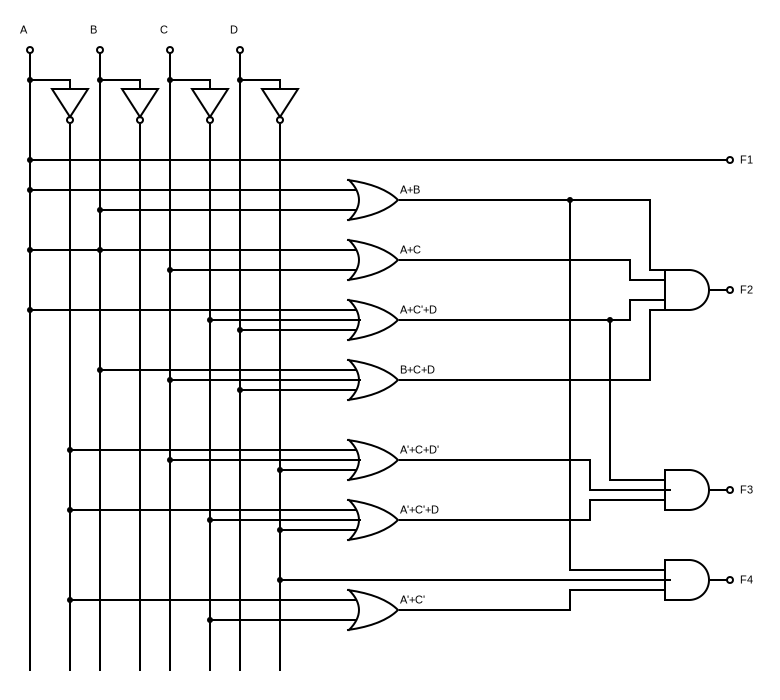
\includegraphics[width=6.30in]{q2_xs3-to-aiken}
	\end{indented}

	\pagebreak

	\noindent
	3. Design a 7-segment decoder for Aiken.
	\begin{indented}{5mm}
		$\begin{array}{c|c|c|c||c|c|c|c|c|c|c||c}
			A & B & C & D & F1 & F2 & F3 & F4 & F5 & F6 & F7 & \#\\
			\hline
			0 & 0 & 0 & 0 & 1 & 1 & 1 & 1 & 1 & 1 & 1 & 0\\ % 0
			0 & 0 & 0 & 1 & 0 & 0 & 0 & 0 & 1 & 1 & 0 & 1\\ % 1
			0 & 0 & 1 & 0 & 1 & 0 & 1 & 1 & 0 & 1 & 1 & 2\\ % 2
			0 & 0 & 1 & 1 & 1 & 0 & 0 & 1 & 1 & 1 & 1 & 3\\ % 3
			0 & 1 & 0 & 0 & 0 & 1 & 0 & 0 & 1 & 1 & 1 & 4\\ % 4
			0 & 1 & 0 & 1 & X & X & X & X & X & X & X & 5\\ % X
			0 & 1 & 1 & 0 & X & X & X & X & X & X & X & 6\\ % X
			0 & 1 & 1 & 1 & X & X & X & X & X & X & X & 7\\ % X
			1 & 0 & 0 & 0 & X & X & X & X & X & X & X & 8\\ % X
			1 & 0 & 0 & 1 & X & X & X & X & X & X & X & 9\\ % X
			1 & 0 & 1 & 0 & X & X & X & X & X & X & X & 10\\ % X
			1 & 0 & 1 & 1 & 1 & 1 & 0 & 1 & 1 & 0 & 1 & 11\\ % 5
			1 & 1 & 0 & 0 & 1 & 1 & 1 & 1 & 1 & 0 & 1 & 12\\ % 6
			1 & 1 & 0 & 1 & 1 & 0 & 0 & 0 & 1 & 1 & 0 & 13\\ % 7
			1 & 1 & 1 & 0 & 1 & 1 & 1 & 1 & 1 & 1 & 1 & 14\\ % 8
			1 & 1 & 1 & 1 & 1 & 1 & 0 & 1 & 1 & 1 & 1 & 15\\ % 9
		\end{array}$
		\includegraphics[width=1.2in]{7-segment-display}
		
		\begin{multicols}{2}
			\begin{karnaugh-map}[4][4][1][(F1) \ CD][AB]
				\minterms{1,4}
				\maxterms{0, 2, 3, 11, 12, 13, 14, 15}
				\terms{5,6,7,8,9,10}{X}
				
				\implicant{1}{5}
				\implicant{4}{6}
			\end{karnaugh-map}\\
			\begin{karnaugh-map}[4][4][1][(F2) \ CD][AB]
				\minterms{1, 2, 3, 13}
				\maxterms{0, 4, 11, 12, 14, 15}
				\terms{5,6,7,8,9,10}{X}
				
				\implicant{1}{7}
				\implicant{3}{6}
				\implicant{1}{9}
			\end{karnaugh-map}\\
			\begin{karnaugh-map}[4][4][1][(F3) \ CD][AB]
				\minterms{1, 3, 4, 11, 13, 15}
				\maxterms{0, 2, 12, 14}
				\terms{5,6,7,8,9,10}{X}
				
				\implicant{1}{11}
				\implicant{4}{6}
			\end{karnaugh-map}\\
			\begin{karnaugh-map}[4][4][1][(F5) \ CD][AB]
				\minterms{2}
				\maxterms{0, 1, 3, 4, 11, 12, 13, 14, 15}
				\terms{5,6,7,8,9,10}{X}
				
				\implicant{2}{6}
			\end{karnaugh-map}\\
			\begin{karnaugh-map}[4][4][1][(F7) \ CD][AB]
				\minterms{1, 13}
				\maxterms{0, 2, 3, 4, 11, 12, 14, 15}
				\terms{5,6,7,8,9,10}{X}
				
				\implicant{1}{9}
			\end{karnaugh-map}\\
			\begin{karnaugh-map}[4][4][1][(F4) \ CD][AB]
				\minterms{1, 4, 13}
				\maxterms{0, 2, 3, 11, 12, 14, 15}
				\terms{5,6,7,8,9,10}{X}
				
				\implicant{1}{9}
				\implicant{4}{6}
			\end{karnaugh-map}\\
			\begin{karnaugh-map}[4][4][1][(F6) \ CD][AB]
				\minterms{11, 12}
				\maxterms{0, 1, 2, 3, 4, 13, 14, 15}
				\terms{5,6,7,8,9,10}{X}
				
				\implicant{12}{8}
				\implicant{8}{10}
			\end{karnaugh-map}
		\end{multicols}
		
		$\begin{aligned}
			\therefore F1 &=((A'C'D)+(A'B))' \\
			&= (A+C+D')(A+B')
		\end{aligned}$
		
		$\begin{aligned}
			\therefore F2 &=((A'D)+(A'C))' \\
			&= (A+D')(A+C')
		\end{aligned}$
		
		$\begin{aligned}
			\therefore F3 &=((D)+(A'B))' \\
			&= (D')(A+B')
		\end{aligned}$
		
		$\begin{aligned}
			\therefore F4 &=((C'D)+(A'B))' \\
			&= (C+D')(A+B')
		\end{aligned}$
		
		$\begin{aligned}
			\therefore F5 &=(A'CD')' \\
			&= (A+C'+D)
		\end{aligned}$
		
		$\begin{aligned}
			\therefore F6 &=((AC'D')+(AB'))' \\
			&= (A'+C+D)(A'+B)
		\end{aligned}$
		
		$\begin{aligned}
			\therefore F7 &=(C'D)' \\
			&= (C+D')
		\end{aligned}$
		
		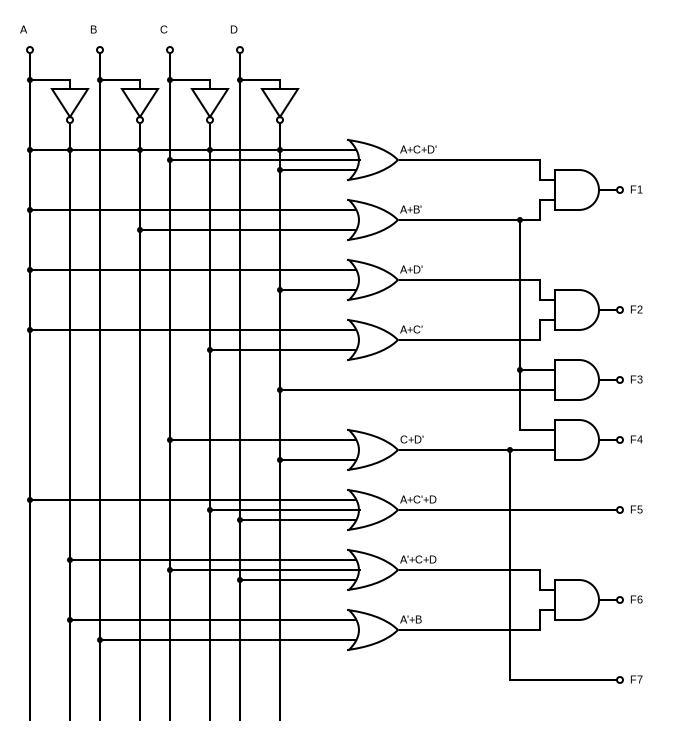
\includegraphics[width=5.5in]{q3_seven-segment}
	\end{indented}
\end{document}
		